\documentclass[12pt,a4paper]{article}

\usepackage[utf8]{inputenc}
\usepackage[T1]{fontenc}
\usepackage{amsmath}
\usepackage{geometry}
\usepackage{booktabs}
\usepackage{graphicx}
\usepackage{xcolor}
\usepackage{float}

\geometry{margin=1in}

\title{Report 2: Linear Regression}
\author{Dao Quy Tung - 2540109}
\date{May 12, 2026}

\begin{document}

\maketitle

\section{Introduction}

The objective of this labwork is to implement linear regression from scratch using gradient descent.
The model is trained on a small CSV dataset and the goal is to find a line that fits the data points.

This labwork contains two parts. The first part trains linear regression using mean squared error. The extra part uses the same model but writes the loss as \(\frac{1}{2}(\hat{y}-y)^2\) and updates the parameters \(w_0\) and \(w_1\) using partial derivatives.

The dataset used in the experiment is:

\begin{table}[H]
\centering
\begin{tabular}{cc}
\toprule
\(x\) & \(y\) \\
\midrule
10 & 55 \\
20 & 80 \\
40 & 100 \\
60 & 120 \\
80 & 150 \\
\bottomrule
\end{tabular}
\caption{Training data from \texttt{lr.csv}.}
\end{table}

\section{Linear Regression Algorithm}

The linear regression model is:

\[
\hat{y} = w_1x + w_0
\]

where \(x\) is the input value, \(y\) is the true value, and \(\hat{y}\) is the predicted value.
The goal is to adjust \(w_0\) and \(w_1\) so that the predicted values are close to the true values.

For the extra part, the loss of one data point is:

\[
L_i = \frac{1}{2}(\hat{y}_i - y_i)^2
\]

Since:

\[
\hat{y}_i = w_1x_i + w_0
\]

the loss can be written as:

\[
L_i = \frac{1}{2}(w_1x_i + w_0 - y_i)^2
\]

The partial derivatives are:

\[
\frac{\partial L_i}{\partial w_0} = w_1x_i + w_0 - y_i
\]

\[
\frac{\partial L_i}{\partial w_1} = x_i(w_1x_i + w_0 - y_i)
\]

The parameters are updated using gradient descent:

\[
w_0 := w_0 - r\frac{\partial J}{\partial w_0}
\]

\[
w_1 := w_1 - r\frac{\partial J}{\partial w_1}
\]

\section{Implementation}

The implementation reads the training data from \texttt{lr.csv}, initializes the model parameters, then repeatedly updates the parameters using gradient descent.

The main steps are:

\begin{enumerate}
  \item Read the input values \(x\) and target values \(y\) from the CSV file.
  \item Initialize the model parameters.
  \item Compute the predicted value \(\hat{y}\) for each data point.
  \item Compute the error between prediction and true value.
  \item Compute the loss and the gradients.
  \item Update the model parameters using the learning rate.
  \item Repeat until the stopping condition is reached.
\end{enumerate}

Two versions were tested:

\begin{table}[H]
\centering
\begin{tabular}{lcc}
\toprule
Version & Initial parameters & Reported loss \\
\midrule
Basic linear regression & \(w=0, b=0\) & Mean squared error \\
Linear regression extras & \(w_0=0, w_1=1\) & Average \(\frac{1}{2}(\hat{y}-y)^2\) \\
\bottomrule
\end{tabular}
\caption{Two implementations used in Labwork 2.}
\end{table}

\section{Experiment Output and Learning Rate Analysis}

The basic experiment was executed with:

\[
w = 0, \quad b = 0, \quad r = 0.0001, \quad threshold = 19
\]

Selected output from the basic experiment:

\begin{table}[H]
\centering
\begin{tabular}{rrrr}
\toprule
Step & \(w\) & \(b\) & Loss \\
\midrule
0 & 0.0000 & 0.0000 & 11265.0000 \\
1 & 1.0140 & 0.0202 & 3468.9149 \\
2 & 1.5371 & 0.0319 & 1394.2838 \\
3 & 1.8069 & 0.0392 & 842.1633 \\
4 & 1.9460 & 0.0442 & 695.1914 \\
5 & 2.0178 & 0.0480 & 656.0318 \\
10000 & 1.7463 & 20.1000 & 229.7248 \\
20000 & 1.5437 & 31.7687 & 90.2109 \\
40000 & 1.3574 & 42.5019 & 27.0606 \\
60000 & 1.2944 & 46.1322 & 19.8358 \\
80000 & 1.2731 & 47.3602 & 19.0092 \\
80833 & 1.2726 & 47.3879 & 19.0000 \\
\bottomrule
\end{tabular}
\caption{Selected output of the basic linear regression experiment.}
\end{table}

The final model is:

\[
\hat{y} = 1.2726x + 47.3879
\]

\begin{figure}[H]
\centering
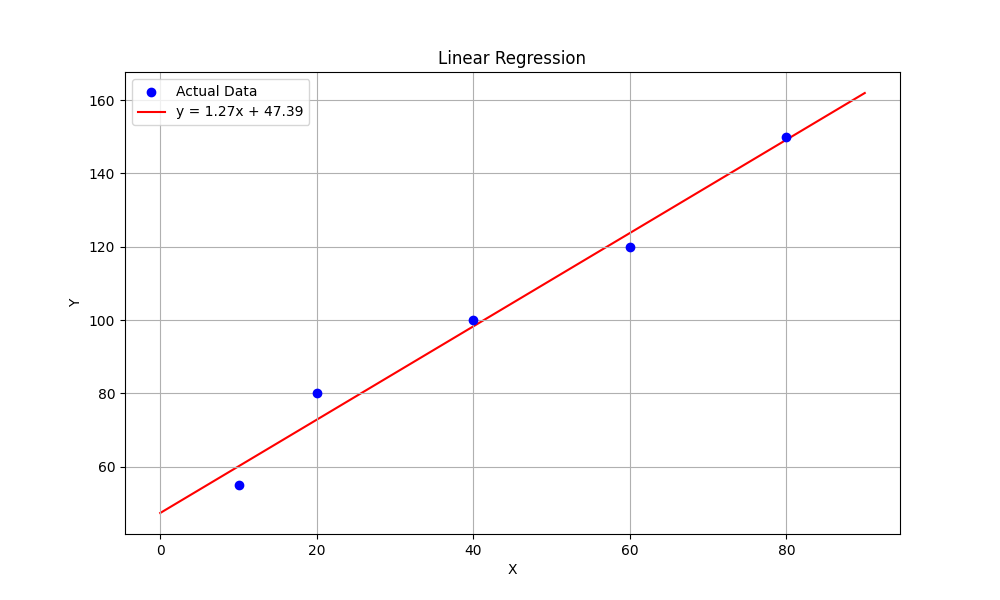
\includegraphics[width=0.85\textwidth]{Linear_regression_result}
\caption{Linear Regression experiment result}
\end{figure}


The extra experiment was executed with:

\[
w_0 = 0, \quad w_1 = 1, \quad r = 0.0001, \quad threshold = 9.5
\]

Selected output from the extra experiment:

\begin{table}[H]
\centering
\begin{tabular}{rrrr}
\toprule
Step & \(w_0\) & \(w_1\) & Loss \(J\) \\
\midrule
0 & 0.0000 & 1.0000 & 1772.5000 \\
10000 & 11.4059 & 1.8972 & 190.8322 \\
20000 & 20.0897 & 1.7464 & 114.9402 \\
40000 & 31.7626 & 1.5438 & 45.1323 \\
60000 & 38.5514 & 1.4260 & 21.5202 \\
80000 & 42.4997 & 1.3575 & 13.5335 \\
100000 & 44.7960 & 1.3176 & 10.8320 \\
140000 & 46.9082 & 1.2809 & 9.6092 \\
160000 & 47.3599 & 1.2731 & 9.5047 \\
161682 & 47.3879 & 1.2726 & 9.5000 \\
\bottomrule
\end{tabular}
\caption{Selected output of the linear regression extra experiment.}
\end{table}

The final model of the extra experiment is also:

\[
\hat{y} = 1.2726x + 47.3879
\]

The final loss values are different because the two experiments report different loss definitions. The basic experiment reports mean squared error, while the extra experiment reports half of the squared error.

\begin{figure}[H]
\centering
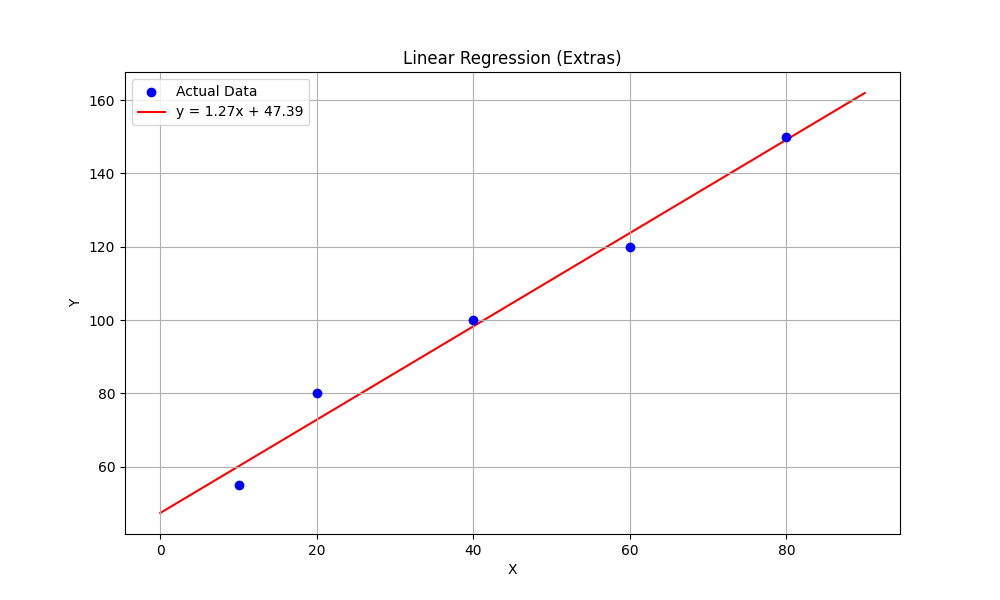
\includegraphics[width=0.85\textwidth]{Linear_regression_extra_result}
\caption{Linear Regression Result for extra experiment}
\end{figure}


\subsection{Learning Rate Comparison}

Different learning rates were also tested on the same dataset:

\begin{table}[H]
\centering
\begin{tabular}{lrrrr}
\toprule
Learning rate & Status & Step & \(w\) & \(b\) \\
\midrule
0.00001 & Not reached & 200000 & 1.5437 & 31.7684 \\
0.00005 & Converged & 161669 & 1.2726 & 47.3879 \\
0.00010 & Converged & 80833 & 1.2726 & 47.3879 \\
0.00050 & Diverged & 27 & 27473.7413 & 477.2201 \\
0.00100 & Diverged & 7 & 25857.6390 & 449.0009 \\
\bottomrule
\end{tabular}
\caption{Effect of different learning rates.}
\end{table}

The learning rate \(0.00001\) is stable, but it is too slow for the selected maximum number of iterations. After 200000 steps, the loss still does not reach the threshold.

The learning rates \(0.00005\) and \(0.0001\) both converge to almost the same final model:

\[
\hat{y} = 1.2726x + 47.3879
\]

However, \(0.0001\) reaches the threshold faster than \(0.00005\). This means that increasing the learning rate can improve convergence speed when the value is still small enough.

The learning rates \(0.0005\) and \(0.001\) are too large. The parameter values become extremely large after only a few steps, and the training diverges. This shows that a larger learning rate is not always better.

\section{Conclusion}

In this labwork, linear regression was implemented from scratch using gradient descent.
Both the basic experiment and the extra experiment reached the same final model:

\[
\hat{y} = 1.2726x + 47.3879
\]

The experiments show that gradient descent can reduce the loss and find a line that follows the general trend of the data. The learning rate is important: a small value makes training slow, a suitable value gives stable convergence, and a large value can make the training diverge.

\end{document}
